\documentclass[1p]{elsarticle_modified}
%\bibliographystyle{elsarticle-num}

%\usepackage[colorlinks]{hyperref}
%\usepackage{abbrmath_seonhwa} %\Abb, \Ascr, \Acal ,\Abf, \Afrak
\usepackage{amsfonts}
\usepackage{amssymb}
\usepackage{amsmath}
\usepackage{amsthm}
\usepackage{scalefnt}
\usepackage{amsbsy}
\usepackage{kotex}
\usepackage{caption}
\usepackage{subfig}
\usepackage{color}
\usepackage{graphicx}
\usepackage{xcolor} %% white, black, red, green, blue, cyan, magenta, yellow
\usepackage{float}
\usepackage{setspace}
\usepackage{hyperref}

\usepackage{tikz}
\usetikzlibrary{arrows}

\usepackage{multirow}
\usepackage{array} % fixed length table
\usepackage{hhline}

%%%%%%%%%%%%%%%%%%%%%
\makeatletter
\renewcommand*\env@matrix[1][\arraystretch]{%
	\edef\arraystretch{#1}%
	\hskip -\arraycolsep
	\let\@ifnextchar\new@ifnextchar
	\array{*\c@MaxMatrixCols c}}
\makeatother %https://tex.stackexchange.com/questions/14071/how-can-i-increase-the-line-spacing-in-a-matrix
%%%%%%%%%%%%%%%

\usepackage[normalem]{ulem}

\newcommand{\msout}[1]{\ifmmode\text{\sout{\ensuremath{#1}}}\else\sout{#1}\fi}
%SOURCE: \msout is \stkout macro in https://tex.stackexchange.com/questions/20609/strikeout-in-math-mode

\newcommand{\cancel}[1]{
	\ifmmode
	{\color{red}\msout{#1}}
	\else
	{\color{red}\sout{#1}}
	\fi
}

\newcommand{\add}[1]{
	{\color{blue}\uwave{#1}}
}

\newcommand{\replace}[2]{
	\ifmmode
	{\color{red}\msout{#1}}{\color{blue}\uwave{#2}}
	\else
	{\color{red}\sout{#1}}{\color{blue}\uwave{#2}}
	\fi
}

\newcommand{\Sol}{\mathcal{S}} %segment
\newcommand{\D}{D} %diagram
\newcommand{\A}{\mathcal{A}} %arc


%%%%%%%%%%%%%%%%%%%%%%%%%%%%%5 test

\def\sl{\operatorname{\textup{SL}}(2,\Cbb)}
\def\psl{\operatorname{\textup{PSL}}(2,\Cbb)}
\def\quan{\mkern 1mu \triangleright \mkern 1mu}

\theoremstyle{definition}
\newtheorem{thm}{Theorem}[section]
\newtheorem{prop}[thm]{Proposition}
\newtheorem{lem}[thm]{Lemma}
\newtheorem{ques}[thm]{Question}
\newtheorem{cor}[thm]{Corollary}
\newtheorem{defn}[thm]{Definition}
\newtheorem{exam}[thm]{Example}
\newtheorem{rmk}[thm]{Remark}
\newtheorem{alg}[thm]{Algorithm}

\newcommand{\I}{\sqrt{-1}}
\begin{document}

%\begin{frontmatter}
%
%\title{Boundary parabolic representations of knots up to 8 crossings}
%
%%% Group authors per affiliation:
%\author{Yunhi Cho} 
%\address{Department of Mathematics, University of Seoul, Seoul, Korea}
%\ead{yhcho@uos.ac.kr}
%
%
%\author{Seonhwa Kim} %\fnref{s_kim}}
%\address{Center for Geometry and Physics, Institute for Basic Science, Pohang, 37673, Korea}
%\ead{ryeona17@ibs.re.kr}
%
%\author{Hyuk Kim}
%\address{Department of Mathematical Sciences, Seoul National University, Seoul 08826, Korea}
%\ead{hyukkim@snu.ac.kr}
%
%\author{Seokbeom Yoon}
%\address{Department of Mathematical Sciences, Seoul National University, Seoul, 08826,  Korea}
%\ead{sbyoon15@snu.ac.kr}
%
%\begin{abstract}
%We find all boundary parabolic representation of knots up to 8 crossings.
%
%\end{abstract}
%\begin{keyword}
%    \MSC[2010] 57M25 
%\end{keyword}
%
%\end{frontmatter}

%\linenumbers
%\tableofcontents
%
\newcommand\colored[1]{\textcolor{white}{\rule[-0.35ex]{0.8em}{1.4ex}}\kern-0.8em\color{red} #1}%
%\newcommand\colored[1]{\textcolor{white}{ #1}\kern-2.17ex	\textcolor{white}{ #1}\kern-1.81ex	\textcolor{white}{ #1}\kern-2.15ex\color{red}#1	}

{\Large $\underline{10_{51}~(K10a_{16})}$}

\setlength{\tabcolsep}{10pt}
\renewcommand{\arraystretch}{1.6}
\vspace{1cm}\begin{tabular}{m{100pt}>{\centering\arraybackslash}m{274pt}}
\multirow{5}{120pt}{
	\centering
	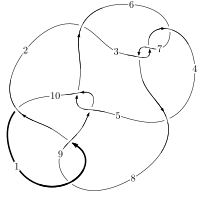
\includegraphics[width=112pt]{../../../GIT/diagram.site/Diagrams/png/135_10_51.png}\\
\ \ \ A knot diagram\footnotemark}&
\allowdisplaybreaks
\textbf{Linearized knot diagam} \\
\cline{2-2}
 &
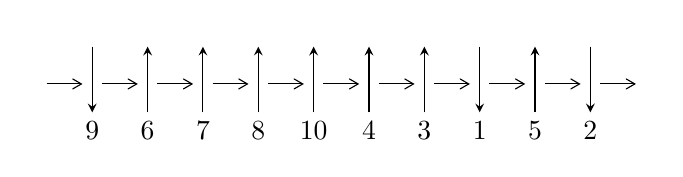
\begin{tikzpicture}[x=20pt, y=17pt]
	% nodes
	\node (C0) at (0, 0) {};
	\node (C1) at (1, 0) {};
	\node (C1U) at (1, +1) {};
	\node (C1D) at (1, -1) {9};

	\node (C2) at (2, 0) {};
	\node (C2U) at (2, +1) {};
	\node (C2D) at (2, -1) {6};

	\node (C3) at (3, 0) {};
	\node (C3U) at (3, +1) {};
	\node (C3D) at (3, -1) {7};

	\node (C4) at (4, 0) {};
	\node (C4U) at (4, +1) {};
	\node (C4D) at (4, -1) {8};

	\node (C5) at (5, 0) {};
	\node (C5U) at (5, +1) {};
	\node (C5D) at (5, -1) {10};

	\node (C6) at (6, 0) {};
	\node (C6U) at (6, +1) {};
	\node (C6D) at (6, -1) {4};

	\node (C7) at (7, 0) {};
	\node (C7U) at (7, +1) {};
	\node (C7D) at (7, -1) {3};

	\node (C8) at (8, 0) {};
	\node (C8U) at (8, +1) {};
	\node (C8D) at (8, -1) {1};

	\node (C9) at (9, 0) {};
	\node (C9U) at (9, +1) {};
	\node (C9D) at (9, -1) {5};

	\node (C10) at (10, 0) {};
	\node (C10U) at (10, +1) {};
	\node (C10D) at (10, -1) {2};
	\node (C11) at (11, 0) {};

	% arrows
	\draw[->,>={angle 60}]
	(C0) edge (C1) (C1) edge (C2) (C2) edge (C3) (C3) edge (C4) (C4) edge (C5) (C5) edge (C6) (C6) edge (C7) (C7) edge (C8) (C8) edge (C9) (C9) edge (C10) (C10) edge (C11) ;	\draw[->,>=stealth]
	(C1U) edge (C1D) (C2D) edge (C2U) (C3D) edge (C3U) (C4D) edge (C4U) (C5D) edge (C5U) (C6D) edge (C6U) (C7D) edge (C7U) (C8U) edge (C8D) (C9D) edge (C9U) (C10U) edge (C10D) ;
	\end{tikzpicture} \\
\hhline{~~} \\& 
\textbf{Solving Sequence} \\ \cline{2-2} 
 &
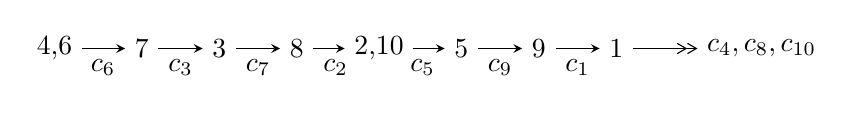
\begin{tikzpicture}[x=28pt, y=7pt]
	% node
	\node (A0) at (-1/8, 0) {4,6};
	\node (A1) at (1, 0) {7};
	\node (A2) at (2, 0) {3};
	\node (A3) at (3, 0) {8};
	\node (A4) at (65/16, 0) {2,10};
	\node (A5) at (41/8, 0) {5};
	\node (A6) at (49/8, 0) {9};
	\node (A7) at (57/8, 0) {1};
	\node (C1) at (1/2, -1) {$c_{6}$};
	\node (C2) at (3/2, -1) {$c_{3}$};
	\node (C3) at (5/2, -1) {$c_{7}$};
	\node (C4) at (7/2, -1) {$c_{2}$};
	\node (C5) at (37/8, -1) {$c_{5}$};
	\node (C6) at (45/8, -1) {$c_{9}$};
	\node (C7) at (53/8, -1) {$c_{1}$};
	\node (A8) at (9, 0) {$c_{4},c_{8},c_{10}$};

	% edge
	\draw[->,>=stealth]	
	(A0) edge (A1) (A1) edge (A2) (A2) edge (A3) (A3) edge (A4) (A4) edge (A5) (A5) edge (A6) (A6) edge (A7) ;
	\draw[->>,>={angle 60}]	
	(A7) edge (A8);
\end{tikzpicture} \\ 

\end{tabular} \\

\footnotetext{
The image of knot diagram is generated by the software ``\textbf{Draw programme}" developed by Andrew Bartholomew(\url{http://www.layer8.co.uk/maths/draw/index.htm\#Running-draw}), where we modified some parts for our purpose(\url{https://github.com/CATsTAILs/LinksPainter}).
}\phantom \\ \newline 
\centering \textbf{Ideals for irreducible components\footnotemark of $X_{\text{par}}$} 
 
\begin{align*}
I^u_{1}&=\langle 
u^{35}+2 u^{34}+\cdots+b-1,\;-2 u^{35}-2 u^{34}+\cdots+a+1,\;u^{36}+2 u^{35}+\cdots- u-1\rangle \\
I^u_{2}&=\langle 
b,\;- u^2+a-1,\;u^3- u^2+2 u-1\rangle \\
\\
\end{align*}
\raggedright * 2 irreducible components of $\dim_{\mathbb{C}}=0$, with total 39 representations.\\
\footnotetext{All coefficients of polynomials are rational numbers. But the coefficients are sometimes approximated in decimal forms when there is not enough margin.}
\newpage
\renewcommand{\arraystretch}{1}
\centering \section*{I. $I^u_{1}= \langle u^{35}+2 u^{34}+\cdots+b-1,\;-2 u^{35}-2 u^{34}+\cdots+a+1,\;u^{36}+2 u^{35}+\cdots- u-1 \rangle$}
\flushleft \textbf{(i) Arc colorings}\\
\begin{tabular}{m{7pt} m{180pt} m{7pt} m{180pt} }
\flushright $a_{4}=$&$\begin{pmatrix}0\\u\end{pmatrix}$ \\
\flushright $a_{6}=$&$\begin{pmatrix}1\\0\end{pmatrix}$ \\
\flushright $a_{7}=$&$\begin{pmatrix}1\\- u^2\end{pmatrix}$ \\
\flushright $a_{3}=$&$\begin{pmatrix}- u\\u^3+u\end{pmatrix}$ \\
\flushright $a_{8}=$&$\begin{pmatrix}u^2+1\\- u^4-2 u^2\end{pmatrix}$ \\
\flushright $a_{2}=$&$\begin{pmatrix}- u^3-2 u\\u^3+u\end{pmatrix}$ \\
\flushright $a_{10}=$&$\begin{pmatrix}2 u^{35}+2 u^{34}+\cdots-4 u-1\\- u^{35}-2 u^{34}+\cdots+7 u^2+1\end{pmatrix}$ \\
\flushright $a_{5}=$&$\begin{pmatrix}u^5+2 u^3+u\\- u^7-3 u^5-2 u^3+u\end{pmatrix}$ \\
\flushright $a_{9}=$&$\begin{pmatrix}u^{23}+10 u^{21}+\cdots+6 u^2-4 u\\u^{35}+2 u^{34}+\cdots- u-1\end{pmatrix}$ \\
\flushright $a_{1}=$&$\begin{pmatrix}u^{35}+u^{34}+\cdots+5 u^2-5 u\\- u^{24}-10 u^{22}+\cdots-6 u^3+4 u^2\end{pmatrix}$\\&\end{tabular}
\flushleft \textbf{(ii) Obstruction class $= -1$}\\~\\
\flushleft \textbf{(iii) Cusp Shapes $= - u^{35}-2 u^{34}-12 u^{33}-22 u^{32}-54 u^{31}-93 u^{30}-72 u^{29}-137 u^{28}+303 u^{27}+296 u^{26}+1632 u^{25}+1737 u^{24}+3476 u^{23}+3488 u^{22}+3688 u^{21}+3414 u^{20}+1095 u^{19}+880 u^{18}-1598 u^{17}-1475 u^{16}-1414 u^{15}-1484 u^{14}+24 u^{13}-396 u^{12}+150 u^{11}+124 u^{10}-166 u^9+148 u^8+30 u^7+48 u^6+66 u^5-17 u^3+24 u^2+14 u+1$}\\~\\
\newpage\renewcommand{\arraystretch}{1}
\flushleft \textbf{(iv) u-Polynomials at the component}\newline \\
\begin{tabular}{m{50pt}|m{274pt}}
Crossings & \hspace{64pt}u-Polynomials at each crossing \\
\hline $$\begin{aligned}c_{1},c_{8}\end{aligned}$$&$\begin{aligned}
&u^{36}-4 u^{35}+\cdots+8 u-1
\end{aligned}$\\
\hline $$\begin{aligned}c_{2},c_{4}\end{aligned}$$&$\begin{aligned}
&u^{36}-2 u^{35}+\cdots+19 u-17
\end{aligned}$\\
\hline $$\begin{aligned}c_{3},c_{6},c_{7}\end{aligned}$$&$\begin{aligned}
&u^{36}+2 u^{35}+\cdots- u-1
\end{aligned}$\\
\hline $$\begin{aligned}c_{5},c_{9}\end{aligned}$$&$\begin{aligned}
&u^{36}+u^{35}+\cdots+12 u+8
\end{aligned}$\\
\hline $$\begin{aligned}c_{10}\end{aligned}$$&$\begin{aligned}
&u^{36}+16 u^{35}+\cdots+24 u+1
\end{aligned}$\\
\hline
\end{tabular}\\~\\
\newpage\renewcommand{\arraystretch}{1}
\flushleft \textbf{(v) Riley Polynomials at the component}\newline \\
\begin{tabular}{m{50pt}|m{274pt}}
Crossings & \hspace{64pt}Riley Polynomials at each crossing \\
\hline $$\begin{aligned}c_{1},c_{8}\end{aligned}$$&$\begin{aligned}
&y^{36}-16 y^{35}+\cdots-24 y+1
\end{aligned}$\\
\hline $$\begin{aligned}c_{2},c_{4}\end{aligned}$$&$\begin{aligned}
&y^{36}-26 y^{35}+\cdots+2461 y+289
\end{aligned}$\\
\hline $$\begin{aligned}c_{3},c_{6},c_{7}\end{aligned}$$&$\begin{aligned}
&y^{36}+30 y^{35}+\cdots+5 y+1
\end{aligned}$\\
\hline $$\begin{aligned}c_{5},c_{9}\end{aligned}$$&$\begin{aligned}
&y^{36}-21 y^{35}+\cdots-784 y+64
\end{aligned}$\\
\hline $$\begin{aligned}c_{10}\end{aligned}$$&$\begin{aligned}
&y^{36}+12 y^{35}+\cdots-516 y+1
\end{aligned}$\\
\hline
\end{tabular}\\~\\
\newpage\flushleft \textbf{(vi) Complex Volumes and Cusp Shapes}
$$\begin{array}{c|c|c}  
\text{Solutions to }I^u_{1}& \I (\text{vol} + \sqrt{-1}CS) & \text{Cusp shape}\\
 \hline 
\begin{aligned}
u &= -0.836039 + 0.127083 I \\
a &= -2.32698 - 0.33462 I \\
b &= \phantom{-}1.30605 - 0.59694 I\end{aligned}
 & \phantom{-}5.69474 - 8.30646 I & \phantom{-}7.90156 + 6.05994 I \\ \hline\begin{aligned}
u &= -0.836039 - 0.127083 I \\
a &= -2.32698 + 0.33462 I \\
b &= \phantom{-}1.30605 + 0.59694 I\end{aligned}
 & \phantom{-}5.69474 + 8.30646 I & \phantom{-}7.90156 - 6.05994 I \\ \hline\begin{aligned}
u &= -0.837370 + 0.074490 I \\
a &= \phantom{-}2.44021 + 0.21899 I \\
b &= -1.346470 + 0.353306 I\end{aligned}
 & \phantom{-}7.51295 - 2.38075 I & \phantom{-}10.48437 + 1.26314 I \\ \hline\begin{aligned}
u &= -0.837370 - 0.074490 I \\
a &= \phantom{-}2.44021 - 0.21899 I \\
b &= -1.346470 - 0.353306 I\end{aligned}
 & \phantom{-}7.51295 + 2.38075 I & \phantom{-}10.48437 - 1.26314 I \\ \hline\begin{aligned}
u &= -0.393001 + 1.122730 I \\
a &= \phantom{-}0.839814 + 0.387760 I \\
b &= -1.315580 - 0.506223 I\end{aligned}
 & \phantom{-}2.65006 + 3.86936 I & \phantom{-}5.24553 - 2.32285 I \\ \hline\begin{aligned}
u &= -0.393001 - 1.122730 I \\
a &= \phantom{-}0.839814 - 0.387760 I \\
b &= -1.315580 + 0.506223 I\end{aligned}
 & \phantom{-}2.65006 - 3.86936 I & \phantom{-}5.24553 + 2.32285 I \\ \hline\begin{aligned}
u &= \phantom{-}0.773363 + 0.051034 I \\
a &= -0.111470 + 0.916399 I \\
b &= \phantom{-}0.224431 - 1.065040 I\end{aligned}
 & \phantom{-}2.25781 + 2.29689 I & \phantom{-}7.21657 - 3.23152 I \\ \hline\begin{aligned}
u &= \phantom{-}0.773363 - 0.051034 I \\
a &= -0.111470 - 0.916399 I \\
b &= \phantom{-}0.224431 + 1.065040 I\end{aligned}
 & \phantom{-}2.25781 - 2.29689 I & \phantom{-}7.21657 + 3.23152 I \\ \hline\begin{aligned}
u &= -0.388829 + 1.191850 I \\
a &= -1.062240 - 0.642876 I \\
b &= \phantom{-}1.360160 + 0.242055 I\end{aligned}
 & \phantom{-}4.08196 - 2.02960 I & \phantom{-}7.16240 + 2.61607 I \\ \hline\begin{aligned}
u &= -0.388829 - 1.191850 I \\
a &= -1.062240 + 0.642876 I \\
b &= \phantom{-}1.360160 - 0.242055 I\end{aligned}
 & \phantom{-}4.08196 + 2.02960 I & \phantom{-}7.16240 - 2.61607 I\\
 \hline 
 \end{array}$$\newpage$$\begin{array}{c|c|c}  
\text{Solutions to }I^u_{1}& \I (\text{vol} + \sqrt{-1}CS) & \text{Cusp shape}\\
 \hline 
\begin{aligned}
u &= -0.741018\phantom{ +0.000000I} \\
a &= -2.98588\phantom{ +0.000000I} \\
b &= \phantom{-}0.930463\phantom{ +0.000000I}\end{aligned}
 & \phantom{-}0.763718\phantom{ +0.000000I} & \phantom{-}8.86550\phantom{ +0.000000I} \\ \hline\begin{aligned}
u &= \phantom{-}0.316713 + 1.230230 I \\
a &= \phantom{-}0.731009 - 0.280668 I \\
b &= -0.073467 - 1.041860 I\end{aligned}
 & -1.35734 + 1.63914 I & \phantom{-}3.47794 - 0.38359 I \\ \hline\begin{aligned}
u &= \phantom{-}0.316713 - 1.230230 I \\
a &= \phantom{-}0.731009 + 0.280668 I \\
b &= -0.073467 + 1.041860 I\end{aligned}
 & -1.35734 - 1.63914 I & \phantom{-}3.47794 + 0.38359 I \\ \hline\begin{aligned}
u &= \phantom{-}0.110839 + 1.278840 I \\
a &= \phantom{-}0.199304 - 0.779639 I \\
b &= -0.585175 - 0.509756 I\end{aligned}
 & -3.23258 + 1.97104 I & \phantom{-}3.37344 - 3.58123 I \\ \hline\begin{aligned}
u &= \phantom{-}0.110839 - 1.278840 I \\
a &= \phantom{-}0.199304 + 0.779639 I \\
b &= -0.585175 + 0.509756 I\end{aligned}
 & -3.23258 - 1.97104 I & \phantom{-}3.37344 + 3.58123 I \\ \hline\begin{aligned}
u &= \phantom{-}0.444529 + 0.543366 I \\
a &= \phantom{-}0.840105 - 0.882584 I \\
b &= -1.105770 - 0.324662 I\end{aligned}
 & \phantom{-}0.90728 + 4.09703 I & \phantom{-}5.30644 - 6.77310 I \\ \hline\begin{aligned}
u &= \phantom{-}0.444529 - 0.543366 I \\
a &= \phantom{-}0.840105 + 0.882584 I \\
b &= -1.105770 + 0.324662 I\end{aligned}
 & \phantom{-}0.90728 - 4.09703 I & \phantom{-}5.30644 + 6.77310 I \\ \hline\begin{aligned}
u &= -0.027017 + 1.315680 I \\
a &= -0.29010 + 1.42344 I \\
b &= \phantom{-}0.625122 + 0.681126 I\end{aligned}
 & -6.47860 - 1.16610 I & -2.74685 + 0.24767 I \\ \hline\begin{aligned}
u &= -0.027017 - 1.315680 I \\
a &= -0.29010 - 1.42344 I \\
b &= \phantom{-}0.625122 - 0.681126 I\end{aligned}
 & -6.47860 + 1.16610 I & -2.74685 - 0.24767 I \\ \hline\begin{aligned}
u &= -0.311343 + 1.279420 I \\
a &= \phantom{-}1.87121 + 1.06972 I \\
b &= -0.965876 + 0.174407 I\end{aligned}
 & -3.22138 - 3.79621 I & \phantom{-}3.52420 + 4.06401 I\\
 \hline 
 \end{array}$$\newpage$$\begin{array}{c|c|c}  
\text{Solutions to }I^u_{1}& \I (\text{vol} + \sqrt{-1}CS) & \text{Cusp shape}\\
 \hline 
\begin{aligned}
u &= -0.311343 - 1.279420 I \\
a &= \phantom{-}1.87121 - 1.06972 I \\
b &= -0.965876 - 0.174407 I\end{aligned}
 & -3.22138 + 3.79621 I & \phantom{-}3.52420 - 4.06401 I \\ \hline\begin{aligned}
u &= \phantom{-}0.335799 + 1.303370 I \\
a &= -0.797336 + 0.066999 I \\
b &= -0.336766 + 1.094920 I\end{aligned}
 & -1.97731 + 6.30262 I & \phantom{-}2.30057 - 5.66674 I \\ \hline\begin{aligned}
u &= \phantom{-}0.335799 - 1.303370 I \\
a &= -0.797336 - 0.066999 I \\
b &= -0.336766 - 1.094920 I\end{aligned}
 & -1.97731 - 6.30262 I & \phantom{-}2.30057 + 5.66674 I \\ \hline\begin{aligned}
u &= \phantom{-}0.543094 + 0.361071 I \\
a &= -0.752914 + 0.836491 I \\
b &= \phantom{-}1.016680 - 0.106012 I\end{aligned}
 & \phantom{-}1.46636 - 0.53351 I & \phantom{-}7.64819 - 0.27613 I \\ \hline\begin{aligned}
u &= \phantom{-}0.543094 - 0.361071 I \\
a &= -0.752914 - 0.836491 I \\
b &= \phantom{-}1.016680 + 0.106012 I\end{aligned}
 & \phantom{-}1.46636 + 0.53351 I & \phantom{-}7.64819 + 0.27613 I \\ \hline\begin{aligned}
u &= -0.372314 + 1.319560 I \\
a &= -1.30924 - 1.37083 I \\
b &= \phantom{-}1.323430 - 0.441863 I\end{aligned}
 & \phantom{-}3.14977 - 6.72875 I & \phantom{-}6.21840 + 3.94329 I \\ \hline\begin{aligned}
u &= -0.372314 - 1.319560 I \\
a &= -1.30924 + 1.37083 I \\
b &= \phantom{-}1.323430 + 0.441863 I\end{aligned}
 & \phantom{-}3.14977 + 6.72875 I & \phantom{-}6.21840 - 3.94329 I \\ \hline\begin{aligned}
u &= \phantom{-}0.210596 + 1.368850 I \\
a &= -0.424656 - 0.451211 I \\
b &= -0.759926 + 0.135831 I\end{aligned}
 & -3.87079 + 2.11524 I & \phantom{-}4.29140 + 1.12167 I \\ \hline\begin{aligned}
u &= \phantom{-}0.210596 - 1.368850 I \\
a &= -0.424656 + 0.451211 I \\
b &= -0.759926 - 0.135831 I\end{aligned}
 & -3.87079 - 2.11524 I & \phantom{-}4.29140 - 1.12167 I \\ \hline\begin{aligned}
u &= -0.365320 + 1.351690 I \\
a &= \phantom{-}1.28028 + 1.56464 I \\
b &= -1.28411 + 0.65656 I\end{aligned}
 & \phantom{-}1.04241 - 12.63140 I & \phantom{-}3.42125 + 8.03158 I\\
 \hline 
 \end{array}$$\newpage$$\begin{array}{c|c|c}  
\text{Solutions to }I^u_{1}& \I (\text{vol} + \sqrt{-1}CS) & \text{Cusp shape}\\
 \hline 
\begin{aligned}
u &= -0.365320 - 1.351690 I \\
a &= \phantom{-}1.28028 - 1.56464 I \\
b &= -1.28411 - 0.65656 I\end{aligned}
 & \phantom{-}1.04241 + 12.63140 I & \phantom{-}3.42125 - 8.03158 I \\ \hline\begin{aligned}
u &= \phantom{-}0.096201 + 1.407940 I \\
a &= \phantom{-}0.333081 + 1.018580 I \\
b &= \phantom{-}0.995297 + 0.496043 I\end{aligned}
 & -5.27687 + 5.74916 I & \phantom{-0.000000 } 0. - 6.40491 I \\ \hline\begin{aligned}
u &= \phantom{-}0.096201 - 1.407940 I \\
a &= \phantom{-}0.333081 - 1.018580 I \\
b &= \phantom{-}0.995297 - 0.496043 I\end{aligned}
 & -5.27687 - 5.74916 I & \phantom{-0.000000 -}0. + 6.40491 I \\ \hline\begin{aligned}
u &= \phantom{-}0.456356\phantom{ +0.000000I} \\
a &= -0.741212\phantom{ +0.000000I} \\
b &= \phantom{-}0.450302\phantom{ +0.000000I}\end{aligned}
 & \phantom{-}0.789103\phantom{ +0.000000I} & \phantom{-}12.7730\phantom{ +0.000000I} \\ \hline\begin{aligned}
u &= -0.157570 + 0.278904 I \\
a &= \phantom{-}0.40346 - 1.83069 I \\
b &= -0.268417 - 0.538256 I\end{aligned}
 & -1.65748 - 0.63628 I & -3.12504 + 1.61784 I \\ \hline\begin{aligned}
u &= -0.157570 - 0.278904 I \\
a &= \phantom{-}0.40346 + 1.83069 I \\
b &= -0.268417 + 0.538256 I\end{aligned}
 & -1.65748 + 0.63628 I & -3.12504 - 1.61784 I\\
 \hline 
 \end{array}$$\newpage\newpage\renewcommand{\arraystretch}{1}
\centering \section*{II. $I^u_{2}= \langle b,\;- u^2+a-1,\;u^3- u^2+2 u-1 \rangle$}
\flushleft \textbf{(i) Arc colorings}\\
\begin{tabular}{m{7pt} m{180pt} m{7pt} m{180pt} }
\flushright $a_{4}=$&$\begin{pmatrix}0\\u\end{pmatrix}$ \\
\flushright $a_{6}=$&$\begin{pmatrix}1\\0\end{pmatrix}$ \\
\flushright $a_{7}=$&$\begin{pmatrix}1\\- u^2\end{pmatrix}$ \\
\flushright $a_{3}=$&$\begin{pmatrix}- u\\u^2- u+1\end{pmatrix}$ \\
\flushright $a_{8}=$&$\begin{pmatrix}u^2+1\\- u^2+u-1\end{pmatrix}$ \\
\flushright $a_{2}=$&$\begin{pmatrix}- u^2-1\\u^2- u+1\end{pmatrix}$ \\
\flushright $a_{10}=$&$\begin{pmatrix}u^2+1\\0\end{pmatrix}$ \\
\flushright $a_{5}=$&$\begin{pmatrix}1\\0\end{pmatrix}$ \\
\flushright $a_{9}=$&$\begin{pmatrix}u^2+1\\0\end{pmatrix}$ \\
\flushright $a_{1}=$&$\begin{pmatrix}0\\u^2- u+1\end{pmatrix}$\\&\end{tabular}
\flushleft \textbf{(ii) Obstruction class $= 1$}\\~\\
\flushleft \textbf{(iii) Cusp Shapes $= 3 u^2-4 u+4$}\\~\\
\newpage\renewcommand{\arraystretch}{1}
\flushleft \textbf{(iv) u-Polynomials at the component}\newline \\
\begin{tabular}{m{50pt}|m{274pt}}
Crossings & \hspace{64pt}u-Polynomials at each crossing \\
\hline $$\begin{aligned}c_{1}\end{aligned}$$&$\begin{aligned}
&(u+1)^3
\end{aligned}$\\
\hline $$\begin{aligned}c_{2},c_{4}\end{aligned}$$&$\begin{aligned}
&u^3- u^2+1
\end{aligned}$\\
\hline $$\begin{aligned}c_{3}\end{aligned}$$&$\begin{aligned}
&u^3+u^2+2 u+1
\end{aligned}$\\
\hline $$\begin{aligned}c_{5},c_{9}\end{aligned}$$&$\begin{aligned}
&u^3
\end{aligned}$\\
\hline $$\begin{aligned}c_{6},c_{7}\end{aligned}$$&$\begin{aligned}
&u^3- u^2+2 u-1
\end{aligned}$\\
\hline $$\begin{aligned}c_{8},c_{10}\end{aligned}$$&$\begin{aligned}
&(u-1)^3
\end{aligned}$\\
\hline
\end{tabular}\\~\\
\newpage\renewcommand{\arraystretch}{1}
\flushleft \textbf{(v) Riley Polynomials at the component}\newline \\
\begin{tabular}{m{50pt}|m{274pt}}
Crossings & \hspace{64pt}Riley Polynomials at each crossing \\
\hline $$\begin{aligned}c_{1},c_{8},c_{10}\end{aligned}$$&$\begin{aligned}
&(y-1)^3
\end{aligned}$\\
\hline $$\begin{aligned}c_{2},c_{4}\end{aligned}$$&$\begin{aligned}
&y^3- y^2+2 y-1
\end{aligned}$\\
\hline $$\begin{aligned}c_{3},c_{6},c_{7}\end{aligned}$$&$\begin{aligned}
&y^3+3 y^2+2 y-1
\end{aligned}$\\
\hline $$\begin{aligned}c_{5},c_{9}\end{aligned}$$&$\begin{aligned}
&y^3
\end{aligned}$\\
\hline
\end{tabular}\\~\\
\newpage\flushleft \textbf{(vi) Complex Volumes and Cusp Shapes}
$$\begin{array}{c|c|c}  
\text{Solutions to }I^u_{2}& \I (\text{vol} + \sqrt{-1}CS) & \text{Cusp shape}\\
 \hline 
\begin{aligned}
u &= \phantom{-}0.215080 + 1.307140 I \\
a &= -0.662359 + 0.562280 I \\
b &= \phantom{-0.000000 } 0\end{aligned}
 & -4.66906 + 2.82812 I & -1.84740 - 3.54173 I \\ \hline\begin{aligned}
u &= \phantom{-}0.215080 - 1.307140 I \\
a &= -0.662359 - 0.562280 I \\
b &= \phantom{-0.000000 } 0\end{aligned}
 & -4.66906 - 2.82812 I & -1.84740 + 3.54173 I \\ \hline\begin{aligned}
u &= \phantom{-}0.569840\phantom{ +0.000000I} \\
a &= \phantom{-}1.32472\phantom{ +0.000000I} \\
b &= \phantom{-0.000000 } 0\end{aligned}
 & -0.531480\phantom{ +0.000000I} & \phantom{-}2.69480\phantom{ +0.000000I}\\
 \hline 
 \end{array}$$\newpage
\newpage\renewcommand{\arraystretch}{1}
\centering \section*{ III. u-Polynomials}
\begin{tabular}{m{50pt}|m{274pt}}
Crossings & \hspace{64pt}u-Polynomials at each crossing \\
\hline $$\begin{aligned}c_{1}\end{aligned}$$&$\begin{aligned}
&((u+1)^3)(u^{36}-4 u^{35}+\cdots+8 u-1)
\end{aligned}$\\
\hline $$\begin{aligned}c_{2},c_{4}\end{aligned}$$&$\begin{aligned}
&(u^3- u^2+1)(u^{36}-2 u^{35}+\cdots+19 u-17)
\end{aligned}$\\
\hline $$\begin{aligned}c_{3}\end{aligned}$$&$\begin{aligned}
&(u^3+u^2+2 u+1)(u^{36}+2 u^{35}+\cdots- u-1)
\end{aligned}$\\
\hline $$\begin{aligned}c_{5},c_{9}\end{aligned}$$&$\begin{aligned}
&u^3(u^{36}+u^{35}+\cdots+12 u+8)
\end{aligned}$\\
\hline $$\begin{aligned}c_{6},c_{7}\end{aligned}$$&$\begin{aligned}
&(u^3- u^2+2 u-1)(u^{36}+2 u^{35}+\cdots- u-1)
\end{aligned}$\\
\hline $$\begin{aligned}c_{8}\end{aligned}$$&$\begin{aligned}
&((u-1)^3)(u^{36}-4 u^{35}+\cdots+8 u-1)
\end{aligned}$\\
\hline $$\begin{aligned}c_{10}\end{aligned}$$&$\begin{aligned}
&((u-1)^3)(u^{36}+16 u^{35}+\cdots+24 u+1)
\end{aligned}$\\
\hline
\end{tabular}\newpage\renewcommand{\arraystretch}{1}
\centering \section*{ IV. Riley Polynomials}
\begin{tabular}{m{50pt}|m{274pt}}
Crossings & \hspace{64pt}Riley Polynomials at each crossing \\
\hline $$\begin{aligned}c_{1},c_{8}\end{aligned}$$&$\begin{aligned}
&((y-1)^3)(y^{36}-16 y^{35}+\cdots-24 y+1)
\end{aligned}$\\
\hline $$\begin{aligned}c_{2},c_{4}\end{aligned}$$&$\begin{aligned}
&(y^3- y^2+2 y-1)(y^{36}-26 y^{35}+\cdots+2461 y+289)
\end{aligned}$\\
\hline $$\begin{aligned}c_{3},c_{6},c_{7}\end{aligned}$$&$\begin{aligned}
&(y^3+3 y^2+2 y-1)(y^{36}+30 y^{35}+\cdots+5 y+1)
\end{aligned}$\\
\hline $$\begin{aligned}c_{5},c_{9}\end{aligned}$$&$\begin{aligned}
&y^3(y^{36}-21 y^{35}+\cdots-784 y+64)
\end{aligned}$\\
\hline $$\begin{aligned}c_{10}\end{aligned}$$&$\begin{aligned}
&((y-1)^3)(y^{36}+12 y^{35}+\cdots-516 y+1)
\end{aligned}$\\
\hline
\end{tabular}
\vskip 2pc
\end{document}